\documentclass{sig-alternate-05-2015}


\begin{document}

\title{TAC AdX competition: Agent NAMM}
\numberofauthors{1}
\author{
% 1st. author
\alignauthor
Alun Meredith\\
       \affaddr{University of Southampton}\\
       \email{am5e15@soton.ac.uk}
}
\maketitle
\begin{abstract}
In this competition we proposed a machine learning based agent; using prediction instead of explicit strategies. Due to the workload and skill-set required to produce such a complex agent the implementation fell short in some areas.

NAMM performed approximately average in a competition dominated by few successful agents with the same strategy of investing in quality early in order to take advantage of no competition later in the game.

Although real world ad exchange agents operate in a way similar to our strategy \cite{edelman2005internet}, in this competition success came from exploiting the structure of the game with simple and effective strategies. 
\end{abstract}


%
% The code below should be generated by the tool at
% http://dl.acm.org/ccs.cfm
% Please copy and paste the code instead of the example below. 
%
\begin{CCSXML}
<ccs2012>
<concept>
<concept_id>10010147.10010178.10010219.10010221</concept_id>
<concept_desc>Computing methodologies~Intelligent agents</concept_desc>
<concept_significance>500</concept_significance>
</concept>
<concept>
<concept_id>10010147.10010257</concept_id>
<concept_desc>Computing methodologies~Machine learning</concept_desc>
<concept_significance>300</concept_significance>
</concept>
<concept>
<concept_id>10002951.10003260.10003282.10003550.10003596</concept_id>
<concept_desc>Information systems~Online auctions</concept_desc>
<concept_significance>300</concept_significance>
</concept>
</ccs2012>
\end{CCSXML}

\ccsdesc[500]{Computing methodologies~Intelligent agents}
\ccsdesc[300]{Computing methodologies~Machine learning}
\ccsdesc[300]{Information systems~Online auctions}



%
% End generated code
%

%
%  Use this command to print the description
%
\printccsdesc

% We no longer use \terms command
%\terms{Theory}

\keywords{TAC AdX; ad exchange;}

\section{Introduction}
The core challenges that face the design of a successful TAC AdX agent are as follows:

\begin{enumerate}
\item Maintaining high reputation. 
\item Maximising end profitability. 
\item Minimising the levels of competition.
\item Ensure 1-3 in an unknown and often unpredictable market. 
\end{enumerate}

To tackle these challenges the design of NAMM was focused on the core theorem that the second price auction is honest\cite{vickrey1961counterspeculation} leading us to our principal of design: 

\newtheorem{theorem}{Principal}
\begin{theorem}
Predict and bid the value of the object being auctioned to NAMM. 
\end{theorem}

In order to implement this principal and maximise our background in data science we treated the task as a machine learning one. Having our agent make predictions, assess the quality of the predictions and adjust future action based on those results. This lead to a highly interconnected system where the action of each part was able to react to the demands of different systems and take actions based on the predictions of different systems. In this way we planned to minimise the need for explicit strategies like many of the agents in the past \cite{tao2015tac} in order to improve flexibility and create a more general solution.  

In practice this was very difficult to implement considering our lack of coding ability. Failure to implement some of the parts to the above strategy an effect on the functions of the rest of the agent due to the interconnection of systems.
 
\section{Agent Design}

\begin{figure*}
\centering
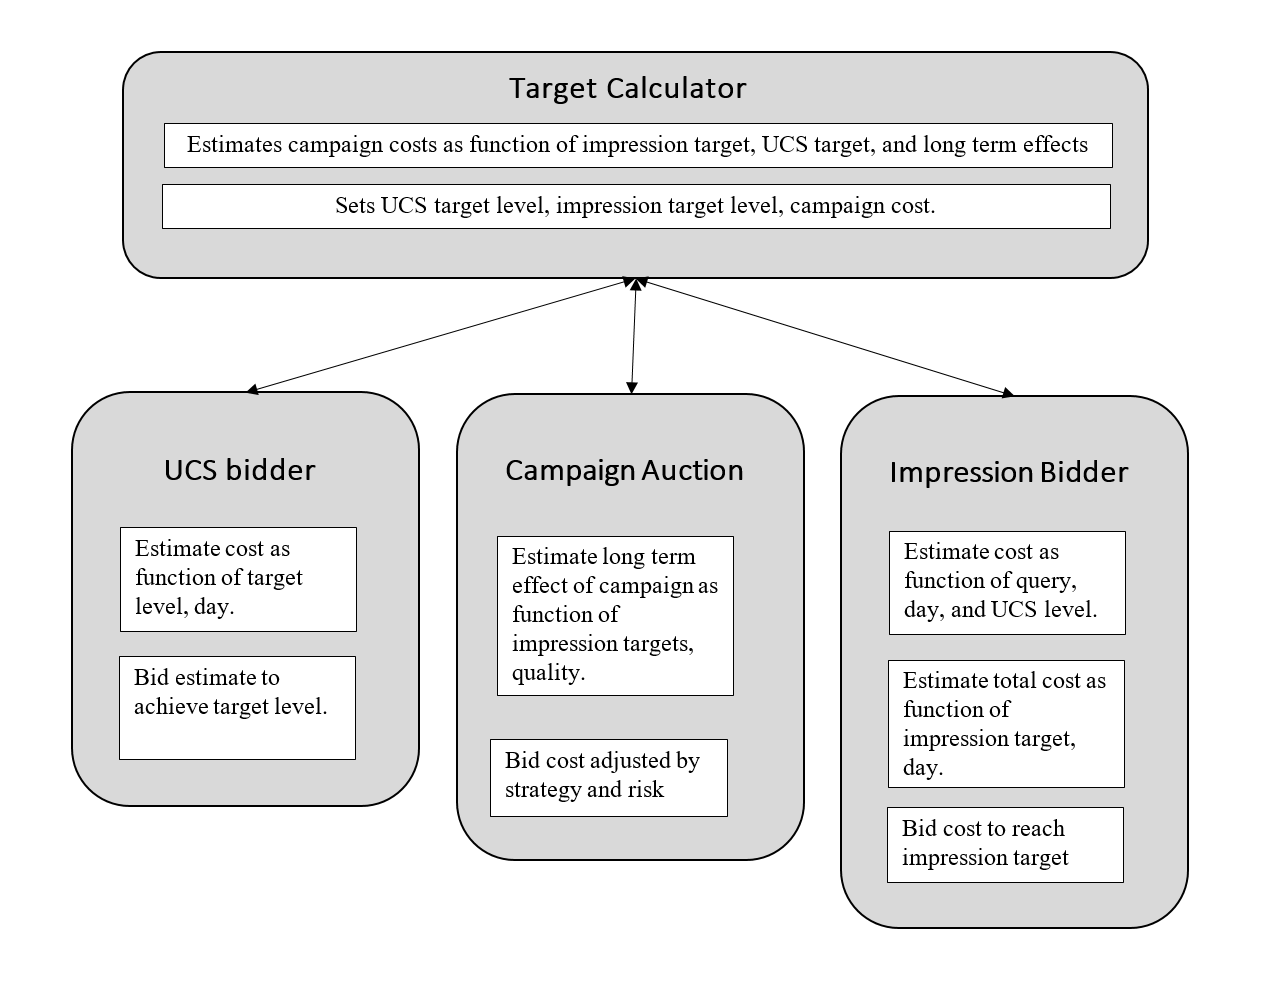
\includegraphics{StructureFlowchart.png}
\caption{Proposed operational structure of NAMM showing the interconnected nature of each bidder, estimating cost over parameters and receiving targets to minimise total cost.}
\label{FlowChart}
\end{figure*}

To implement principal 1 and our design philosophies the design structure in figure \ref{FlowChart} was proposed. The different bidding auctions estimate the costs to achieve different targets in each of their auctions while a target calculator queries these estimates to produce the best permutation of targets in order to maximise profit. 

The primary challenge to this strategy is accurate estimation of the costs faced by each of the 3 auctions especially when predicting the future. To overcome this challenge detailed performance loggers were constructed in order to have the data to make predictions with, test and improve the performance of those predictions.

The areas of the project which were my sole responsibility were: the overall design of the agent (Fig.\ref{FlowChart}), the target calculator, the campaign logger and the campaign bidder.
\subsection{Campaign Auction}
The campaign bidding auction relied on the target calculator to estimate a cost for each campaign before applying some modifiers in order to improve the bids. Here there were 3 main explicit strategies: 

\begin{enumerate}
\item Starting Strategy (during the first campaign)
\item Quality Recovery Strategy (When quality < 1)
\item Profit Strategy (Otherwise)
\end{enumerate}

The starting strategy applied a $0.8,1.5$ and $2.0\times$ modifiers to long,medium and short campaigns respectively. This compensates for increased impression competition and importance of completing the first campaign with a high quality score. Long campaigns have a lower bid because if quality does fall from the first auction ongoing campaigns can recover quality. \textbf{[CITE STUDENT PAPER]}

The quality recovery strategy multiplies the bid by the square of NAMM's quality. The campaign bid multiplied by the quality gives the agent's effective bid enabling NAMM to compete with high quality users fairly at the expense of profit. Multiplying this bid by quality again demonstrates desperation to have a campaign in order to recover quality, this desperation becomes greater and greater the further from $Q=1$. 

Future work for this strategy considered was to have quality recovery effect based on the past experiences of NAMM to complete the campaigns otherwise this strategy risks producing a negative feedback loop where quality is low  but NAMM continues to loose money on unprofitable campaigns. 

The profit maximising strategy provided the base bid for which the other two systems augmented. Here the estimated cost to run a campaign was taken and multiplied by $\times 1.1$ to quantify the risk willing to be taken on a campaign.

Finally a minimum and maximum acceptable bid was calculated. If the bid was below the 30th percentile of unprofitable bids it was changed to that lower bound. The minimum bid was an estimate of the lowest campaign bid which could still be profitable. This was a conservative boundary because it didn't take into account the state of the system like the target calculator did but prevented anomalous results based on past experiences. 

If the bid was above the 90th percentile of successful campaign bids it was set to the highest possible bid. This maximum was deemed the highest bid where it is still plausible we could win the campaign, otherwise the highest possible bid is set in order to take advantage of any randomly allocated campaigns NAMM may earn. 
 
For other effects such as competition the campaign auction relied on the estimation algorithms to account for this, for example competition increases the cost to get an impression in that query. 

\subsection{Logging}
The core to approaching TAC AdX as a machine learning one is the idea of logging and storing the results of each campaign in order to estimate and learn strategies instead of speculating. This provided two main opportunities. It allowed the parameters of NAMM to not be hard coded but learnt or at least manually adjusted through quantitative testing. Secondly it allowed NAMM to dynamically adjust its estimates to compensate for systematic errors. Thirdly it allowed NAMM to learn default values for estimates to be used at the start of the game. I.e. the lower and upper bounds start each game trained on previous games and slowly have more and more of its value based on the current game.  
\section{Implementation}
As mentioned in the introduction some of the design strategies, specifically the estimations of ucs and impressions as a function of other variables were not implemented, instead these auctions estimated bids internally without communicating predictions to other auctions. 
This unfortunately broke the ability of the target calculator to effectively estimate costs and the campaign auction bidder's ability to use this information. The implemented impression bidding strategy was based on estimate of reserve price, popularity in the sector and ucs level. 

The final campaign auction used a simple algorithm to calculate the initial bid price, before augmentation. At the start of the game NAMM would bid random values until successful and then use the pool of successful campaign bids and big randomly around those values. This initial bidding was changed during the game to start at a high bid and slowly bid less and less per impression until successful. This was changed after observing how early campaigns were generally detrimental to quality. 

Over the course of the competition many minor adjustments were made, perceptrons were added to each of the bids, the impression bidder was prevented from bidding on unknown campaigns due to their expense and the impression price estimate was rescaled to become more accurate. Although these changes meant a lot of errors and debugging the outcome was positive and NAMM won its penultimate game (116).

\begin{figure}
\centering
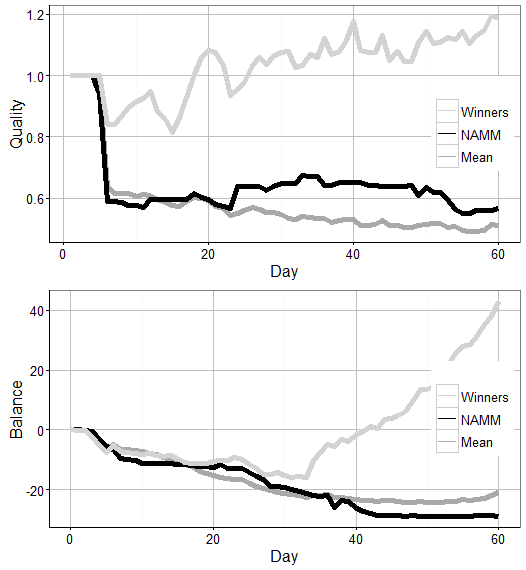
\includegraphics[width = .7\linewidth]{AvsPlot.png}
\caption{The mean performance in terms of Quality and balance of: the Winner of each game, the average of all players in the game and NAMM}
\label{AvsPlot}
\end{figure}
From the results of the game it is easy to classify the agents into two categories, those which maintained quality and those which didn't. Those which maintained quality continued playing the game for its duration, getting great profits or great losses. However those who failed to maintain quality like NAMM tended to have very little profit or loss, participating in a few campaigns. Therefore although NAMM didn't perform well it also rarely performed particularly poorly. 

Over the course of the competition there were three main trends in NAMMs actions. Firstly and primarily NAMM failed to maintain quality during the first campaign. At day 6 the average quality was negative and didn't recover (\ref{AvsPlot}). It is likely an error in the impression bidding algorithm trying to account for different sector competition levels. 

Few campaigns were profitable, having one of the highest average price per impressions especially when considering the number of impressions achieved was often too low to maintain quality (\ref{PriceBar}). NAMM generally was consistent with the probility distribution of other agents  (\ref{PriceHist}) however there was a cluster of very expensive impressions (0.1 - 1 per impression) which likely caused much of the overpaying issues encountered. During the game a cap was introduced to prevent these kinds of bids from continuing to occur. 

Lastly NAMM often failed to get many or any campaigns. For many of the games this was due to a bug introduced during the course of the competition which prevented the agent from bidding on campaigns. In addition low quality level made earning campaigns very difficult. Finally the reliance on winning a number of campaigns to provide training data for the campaign bidder would have had a large impact.     

Winning agents tended to follow a fixed formula (\ref{AvsPlot}). Making a loss during the first section of the game, investing to improve quality quality, then during the latter stages of the game taking advantage of little/no competition to earn large amounts of profit.

\begin{figure}
\centering
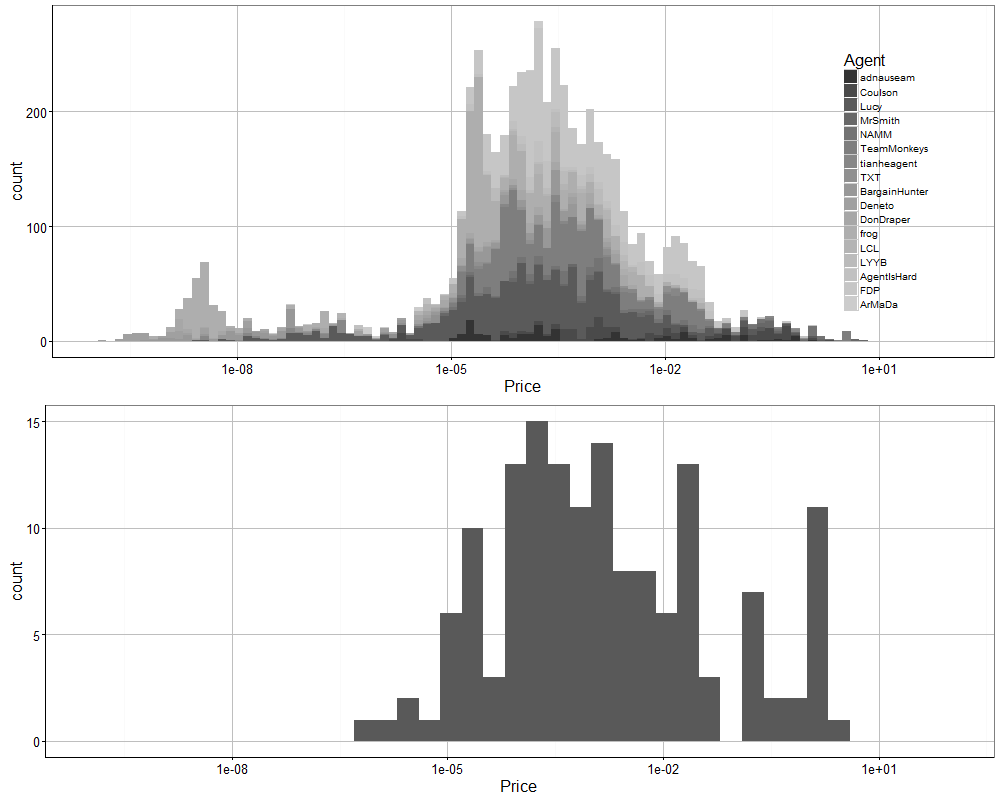
\includegraphics[width = .9\linewidth]{PriceHist.png}
\caption{Histogram of price per impression paid by each of the agents (top) and by NAMM specifically (bottom)}
\label{PriceHist}
\end{figure}

\begin{figure}
\centering
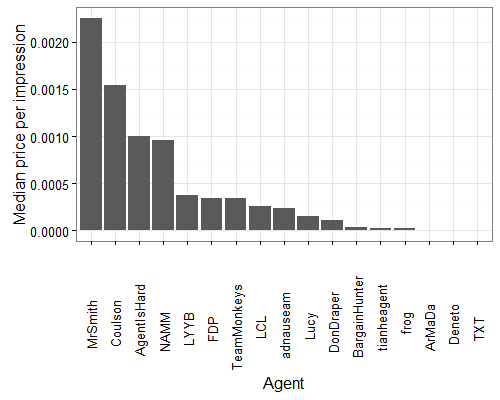
\includegraphics[width = .9\linewidth]{PriceBar.png}
\caption{Bar chart comparison of the median price paid by each of the agents in descending order.}
\label{PriceBar}
\end{figure}


\section{Conclusions}
In hindsight our strategy was too ambitious. A flexible predictive based agent has a very high ceiling but considering the programming knowledge and motivation levels of members of our team it was an impractical goal.  	

Had our strategy been implemented completely it would still have faced challenges, learning dependent strategies are slow to react to the game state and interconnected structure is less stable to flaws in calculations.

Based on the results of the competition I theorise a simple strategy which heavily invests in the first campaign to get high quality. Doesn't bid on campaigns for the first half of the game, waiting for reduced competition before bidding on campaigns and impressions that do not compete with campaigns of other agents. Bidding a maximum of the budget per impression except to guarantee completion of the campaign and a distribution of impressions through multiple ongoing campaigns based on the impressions per day required to fulfil those targets. 

I believe a machine learning based agent is achievable in the time frame of this competition but would revolve much more around having simpler systems with an emphasis on training the model and having better defaults for early stages of the game where learning cannot be applied. 
\section{Acknowledgements}
I would like to take this opportunity to thank my team mates: Miguel Ballesteros Mesa, Manuel Llamas Fernandez and Nicola Vitale for their work on this project as well as the TAC team whom produced the game and sample agent: Yishay Mansour, Mariano Schain and Tomer Greenwald.
\bibliographystyle{abbrv}
\bibliography{sigproc}  % sigproc.bib is the name of the
\appendix
\section{Graph of all games}
\begin{figure*}
\centering
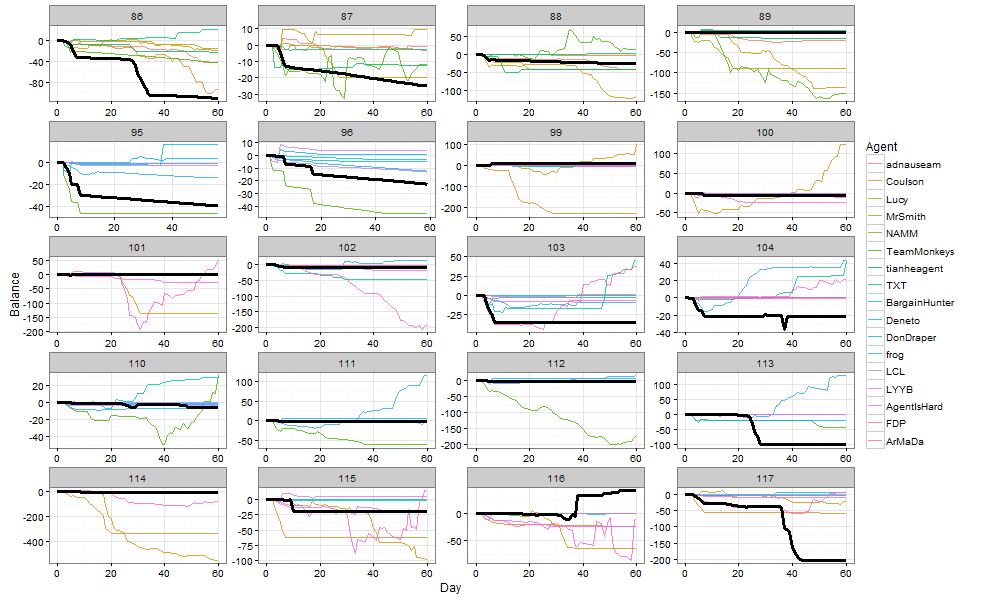
\includegraphics[width = .9\linewidth]{appendix1.png}
\caption{Appendix 1 showing the balance over each game which NAMM participated in. The black line shows the performance of NAMM and the coloured lines the other agents}
\label{Appendix1}
\end{figure*}
\begin{figure*}
\centering
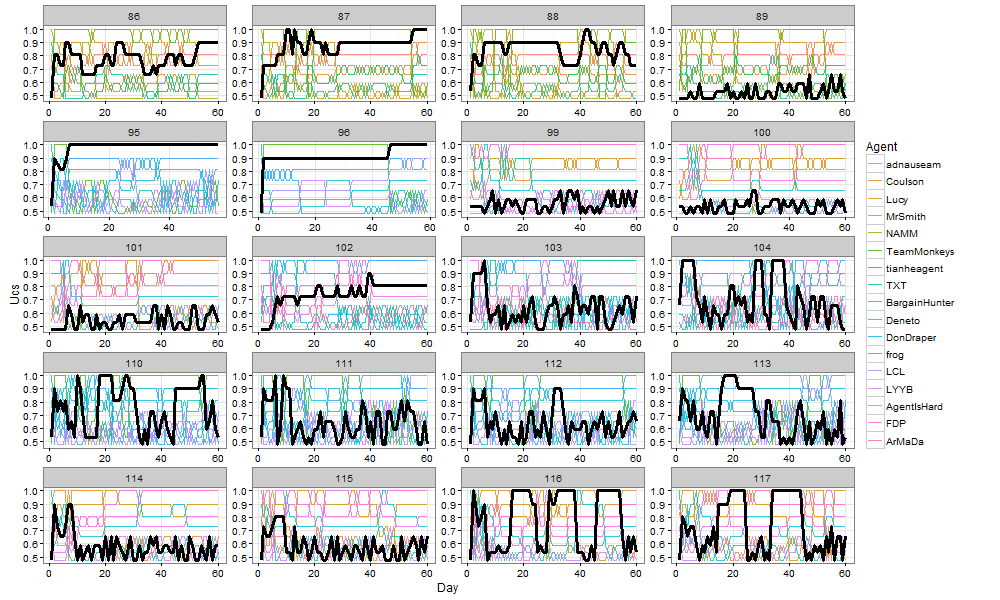
\includegraphics[width = .9\linewidth]{appendix2.png}
\caption{UCS level over each game which NAMM participated in. The black line shows the performance of NAMM and the coloured lines the other agents}
\label{Appendix2}
\end{figure*}
\begin{figure*}
\centering
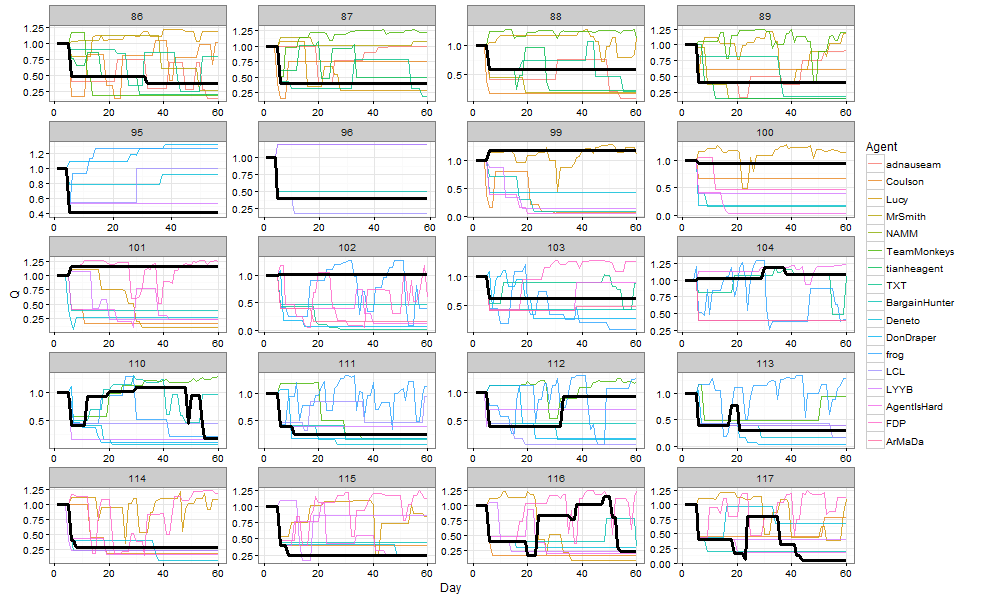
\includegraphics[width = .9\linewidth]{appendix3.png}
\caption{Quality level over each game which NAMM participated in. The black line shows the performance of NAMM and the coloured lines the other agents}
\label{Appendix3}
\end{figure*}

\begin{figure*}
\centering
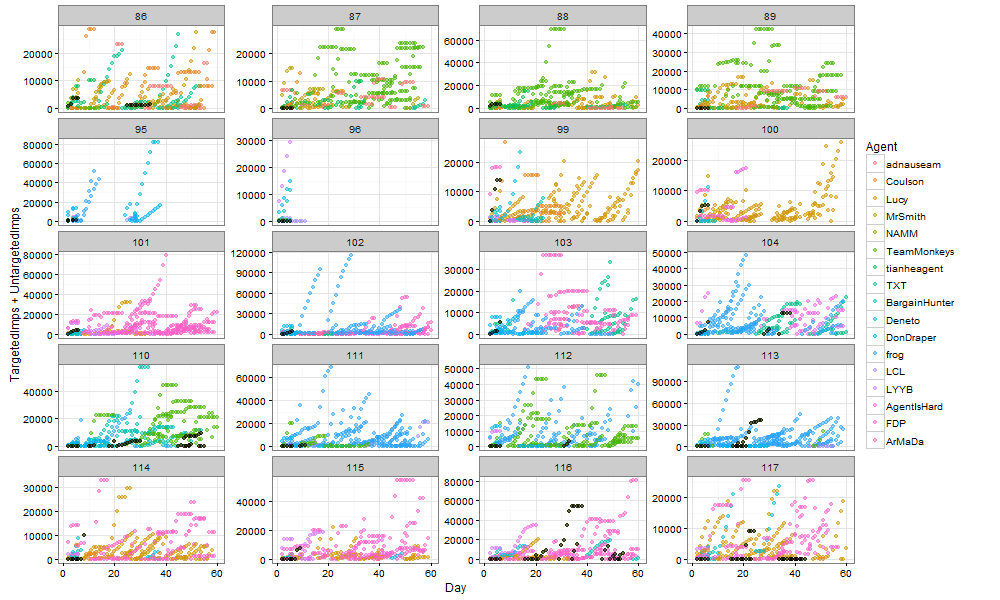
\includegraphics[width = .9\linewidth]{appendix4.png}
\caption{Number of impressions per day over time for each game NAMM participated in. The black line shows performance of NAMM and the coloured lines the other agents}
\label{Appendix4}
\end{figure*}
\end{document}
